
\documentclass[letterpaper,hide notes,xcolor={table,svgnames},pdftex,10pt]{beamer}
\def\showexamples{t}


%\usepackage[svgnames]{xcolor}

%% Demo talk
%\documentclass[letterpaper,notes=show]{beamer}

\usecolortheme{crane}
\setbeamertemplate{navigation symbols}{}

\usetheme{MyPittsburgh}
%\usetheme{Frankfurt}

%\usepackage{tipa}

\usepackage{hyperref}
\usepackage{graphicx,xspace}
\usepackage[normalem]{ulem}
\usepackage{multicol}
\usepackage{amsmath,amssymb,amsthm,graphicx,xspace}
\newcommand\SF[1]{$\bigstar$\footnote{SF: #1}}

\usepackage[default]{sourcesanspro}
\usepackage[T1]{fontenc}
\usepackage[scaled]{beramono}
\usepackage{tikzpagenodes}

\newcounter{tmpnumSlide}
\newcounter{tmpnumNote}


% old question code
%\newcommand\question[1]{{$\bigstar$ \small \onlySlide{2}{#1}}}
% \newcommand\nquestion[1]{\ifdefined \presentationonly \textcircled{?} \fi \note{\par{\Large \textbf{?}} #1}}
% \newcommand\nanswer[1]{\note{\par{\Large \textbf{A}} #1}}


 \newcommand\mnote[1]{%
   \addtocounter{tmpnumSlide}{1}
   \ifdefined\showcues {~\tiny\fbox{\arabic{tmpnumSlide}}}\fi
   \note{\setlength{\parskip}{1ex}\addtocounter{tmpnumNote}{1}\textbf{\Large \arabic{tmpnumNote}:} {#1\par}}}

\newcommand\mmnote[1]{\note{\setlength{\parskip}{1ex}#1\par}}

%\newcommand\mnote[2][]{\ifdefined\handoutwithnotes {~\tiny\fbox{#1}}\fi
% \note{\setlength{\parskip}{1ex}\textbf{\Large #1:} #2\par}}

%\newcommand\mnote[2][]{{\tiny\fbox{#1}} \note{\setlength{\parskip}{1ex}\textbf{\Large #1:} #2\par}}

\newcommand\mquestion[2]{{~\color{red}\fbox{?}}\note{\setlength{\parskip}{1ex}\par{\Large \textbf{?}} #1} \note{\setlength{\parskip}{1ex}\par{\Large \textbf{A}} #2\par}\ifdefined \presentationonly \pause \fi}

\newcommand\blackboard[1]{%
\ifdefined   \showblackboard
  {#1}
  \else {\begin{center} \fbox{\colorbox{blue!30}{%
         \begin{minipage}{.95\linewidth}%
           \hspace{\stretch{1}} Some space intentionally left blank; done at the blackboard.%
         \end{minipage}}}\end{center}}%
         \fi%
}



%\newcommand\q{\tikz \node[thick,color=black,shape=circle]{?};}
%\newcommand\q{\ifdefined \presentationonly \textcircled{?} \fi}

\usepackage{listings}
\lstset{basicstyle=\footnotesize\ttfamily,
	breaklines=true,
	aboveskip=15pt,
  	belowskip=15pt,
	frame=lines,
	numbers=left, basicstyle=\scriptsize, numberstyle=\tiny, stepnumber=0, numbersep=2pt
}

\usepackage{siunitx}
\newcommand\sius[1]{\num[group-separator = {,}]{#1}\si{\micro\second}}
\newcommand\sims[1]{\num[group-separator = {,}]{#1}\si{\milli\second}}
\newcommand\sins[1]{\num[group-separator = {,}]{#1}\si{\nano\second}}
\sisetup{group-separator = {,}, group-digits = true}

%% -------------------- tikz --------------------
\usepackage{tikz}
\usetikzlibrary{positioning}
\usetikzlibrary{arrows,backgrounds,automata,decorations.shapes,decorations.pathmorphing,decorations.markings,decorations.text,decorations.pathreplacing}

\tikzstyle{place}=[circle,draw=blue!50,fill=blue!20,thick, inner sep=0pt,minimum size=6mm]
\tikzstyle{transition}=[rectangle,draw=black!50,fill=black!20,thick, inner sep=0pt,minimum size=4mm]

\tikzstyle{block}=[rectangle,draw=black, thick, inner sep=5pt]
\tikzstyle{bullet}=[circle,draw=black, fill=black, thin, inner sep=2pt]

\tikzstyle{pre}=[<-,shorten <=1pt,>=stealth',semithick]
\tikzstyle{post}=[->,shorten >=1pt,>=stealth',semithick]
\tikzstyle{bi}=[<->,shorten >=1pt,shorten <=1pt, >=stealth',semithick]

\tikzstyle{mut}=[-,>=stealth',semithick]

\tikzstyle{treereset}=[dashed,->, shorten >=1pt,>=stealth',thin]

\usepackage{ifmtarg}
\usepackage{xifthen}
\makeatletter
% new counter to now which frame it is within the sequence
\newcounter{multiframecounter}
% initialize buffer for previously used frame title
\gdef\lastframetitle{\textit{undefined}}
% new environment for a multi-frame
\newenvironment{multiframe}[1][]{%
\ifthenelse{\isempty{#1}}{%
% if no frame title was set via optional parameter,
% only increase sequence counter by 1
\addtocounter{multiframecounter}{1}%
}{%
% new frame title has been provided, thus
% reset sequence counter to 1 and buffer frame title for later use
\setcounter{multiframecounter}{1}%
\gdef\lastframetitle{#1}%
}%
% start conventional frame environment and
% automatically set frame title followed by sequence counter
\begin{frame}%
\frametitle{\lastframetitle~{\normalfont(\arabic{multiframecounter})}}%
}{%
\end{frame}%
}
\makeatother

\makeatletter
\newdimen\tu@tmpa%
\newdimen\ydiffl%
\newdimen\xdiffl%
\newcommand\ydiff[2]{%
    \coordinate (tmpnamea) at (#1);%
    \coordinate (tmpnameb) at (#2);%
    \pgfextracty{\tu@tmpa}{\pgfpointanchor{tmpnamea}{center}}%
    \pgfextracty{\ydiffl}{\pgfpointanchor{tmpnameb}{center}}%
    \advance\ydiffl by -\tu@tmpa%
}
\newcommand\xdiff[2]{%
    \coordinate (tmpnamea) at (#1);%
    \coordinate (tmpnameb) at (#2);%
    \pgfextractx{\tu@tmpa}{\pgfpointanchor{tmpnamea}{center}}%
    \pgfextractx{\xdiffl}{\pgfpointanchor{tmpnameb}{center}}%
    \advance\xdiffl by -\tu@tmpa%
}
\makeatother
\newcommand{\copyrightbox}[3][r]{%
\begin{tikzpicture}%
\node[inner sep=0pt,minimum size=2em](ciimage){#2};
\usefont{OT1}{phv}{n}{n}\fontsize{4}{4}\selectfont
\ydiff{ciimage.south}{ciimage.north}
\xdiff{ciimage.west}{ciimage.east}
\ifthenelse{\equal{#1}{r}}{%
\node[inner sep=0pt,right=1ex of ciimage.south east,anchor=north west,rotate=90]%
{\raggedleft\color{black!50}\parbox{\the\ydiffl}{\raggedright{}#3}};%
}{%
\ifthenelse{\equal{#1}{l}}{%
\node[inner sep=0pt,right=1ex of ciimage.south west,anchor=south west,rotate=90]%
{\raggedleft\color{black!50}\parbox{\the\ydiffl}{\raggedright{}#3}};%
}{%
\node[inner sep=0pt,below=1ex of ciimage.south west,anchor=north west]%
{\raggedleft\color{black!50}\parbox{\the\xdiffl}{\raggedright{}#3}};%
}
}
\end{tikzpicture}
}


%% --------------------

%\usepackage[excludeor]{everyhook}
%\PushPreHook{par}{\setbox0=\lastbox\llap{MUH}}\box0}

%\vspace*{\stretch{1}

%\setbox0=\lastbox \llap{\textbullet\enskip}\box0}

\setlength{\parskip}{\fill}

\newcommand\noskips{\setlength{\parskip}{1ex}}
\newcommand\doskips{\setlength{\parskip}{\fill}}

\newcommand\xx{\par\vspace*{\stretch{1}}\par}
\newcommand\xxs{\par\vspace*{2ex}\par}
\newcommand\tuple[1]{\langle #1 \rangle}
\newcommand\code[1]{{\sf \footnotesize #1}}
\newcommand\ex[1]{\uline{Example:} \ifdefined \presentationonly \pause \fi
  \ifdefined\showexamples#1\xspace\else{\uline{\hspace*{2cm}}}\fi}

\newcommand\ceil[1]{\lceil #1 \rceil}


\AtBeginSection[]
{
   \begin{frame}
       \frametitle{Outline}
       \tableofcontents[currentsection]
   \end{frame}
}



\pgfdeclarelayer{edgelayer}
\pgfdeclarelayer{nodelayer}
\pgfsetlayers{edgelayer,nodelayer,main}

\tikzstyle{none}=[inner sep=0pt]
\tikzstyle{rn}=[circle,fill=Red,draw=Black,line width=0.8 pt]
\tikzstyle{gn}=[circle,fill=Lime,draw=Black,line width=0.8 pt]
\tikzstyle{yn}=[circle,fill=Yellow,draw=Black,line width=0.8 pt]
\tikzstyle{empty}=[circle,fill=White,draw=Black]
\tikzstyle{bw} = [rectangle, draw, fill=blue!20, 
    text width=4em, text centered, rounded corners, minimum height=2em]
    
    \newcommand{\CcNote}[1]{% longname
	This work is licensed under the \textit{Creative Commons #1 3.0 License}.%
}
\newcommand{\CcImageBy}[1]{%
	\includegraphics[scale=#1]{creative_commons/cc_by_30.pdf}%
}
\newcommand{\CcImageSa}[1]{%
	\includegraphics[scale=#1]{creative_commons/cc_sa_30.pdf}%
}
\newcommand{\CcImageNc}[1]{%
	\includegraphics[scale=#1]{creative_commons/cc_nc_30.pdf}%
}
\newcommand{\CcGroupBySa}[2]{% zoom, gap
	\CcImageBy{#1}\hspace*{#2}\CcImageNc{#1}\hspace*{#2}\CcImageSa{#1}%
}
\newcommand{\CcLongnameByNcSa}{Attribution-NonCommercial-ShareAlike}

\newenvironment{changemargin}[1]{% 
  \begin{list}{}{% 
    \setlength{\topsep}{0pt}% 
    \setlength{\leftmargin}{#1}% 
    \setlength{\rightmargin}{1em}
    \setlength{\listparindent}{\parindent}% 
    \setlength{\itemindent}{\parindent}% 
    \setlength{\parsep}{\parskip}% 
  }% 
  \item[]}{\end{list}} 





\title{Lecture 4 --- Rust: Breaking the Rules for Fun and Performance  }

\author{Jeff Zarnett \\ \small \texttt{jzarnett@uwaterloo.ca}}
\institute{Department of Electrical and Computer Engineering \\
  University of Waterloo}
\date{\today}


\begin{document}

\begin{frame}
  \titlepage

 \end{frame}
 

\begin{frame}
\frametitle{Breaking Some Rules}

Previously: mutex is not compatible with our single-ownership model.

We need multiple threads to have access to the mutex.

Background required: smart pointers, reference counting.

\end{frame}


\begin{frame}
\frametitle{Smart Pointers}
We know about pointers from C/\CPP; you may have also seen smart pointers.

We'll talk about two kinds of smart pointer right now, the Box and the Reference-Counting type.

\end{frame}


\begin{frame}
\frametitle{The Box}

The \texttt{Box<T>} is an easy way to put some data on the heap rather than the stack.

\begin{center}
	
\includegraphics[width=0.5\textwidth]{images/amazonbox.jpg}
\end{center}

You create a Box with \texttt{Box::new(...)} .
\end{frame}


\begin{frame}
\frametitle{Reference Counting}

The reference counted smart pointer, however, is the thing that allows for shared ownership

\begin{center}
	
\includegraphics[width=0.4\textwidth]{images/countvoncount.png}
\end{center}

The value only goes away when the last reference to it is dropped.

To make a reference-counted object, use type \texttt{Rc<T>}.

\end{frame}


\begin{frame}
\frametitle{Reference Counting}
If you want to make another reference to the same object, use \texttt{clone()}

When references are dropped, the count decreases.

It is important to note that reference types can leak memory!

\begin{center}
	
\includegraphics[width=0.4\textwidth]{images/reference-cycle.jpg}
\end{center}

\end{frame}


\begin{frame}
\frametitle{Reference Counting}

Unlike \CPP's analogous \texttt{shared\_ptr} you can't keep a reference after the \texttt{Rc} goes out of scope.

Right, so we have everything we need now to pass the mutex around, right? 

Well, almost. \texttt{Rc<T>} won't work when we try to pass it between threads.

The compiler says it cannot be sent between threads safely. 

\end{frame}


\begin{frame}
\frametitle{Atomic Reference Count}

We need the \textit{atomic} reference counted type, which is \texttt{Arc<T>}. 

It is perhaps slightly slower than the regular reference counted type.\\
\quad But exactly what we need here.

\end{frame}


\begin{frame}[fragile]
\frametitle{SIGINT Handler}

Let's catch a SIGINT with an atomic type.

\begin{lstlisting}[language=Rust]
use std::sync::Arc;
use std::sync::atomic::{AtomicBool, Ordering};

fn main() {
   let quit = Arc::new(Mutex::new(false));
    let handler_quit = Arc::clone(&quit);
    ctrlc::set_handler(move || {
        let mut b = handler_quit.lock().unwrap();
        *b = true;
    }).expect("Error setting Ctrl-C handler");
 
    while !(*quit.lock().unwrap()) {
    	// Do things
    }
}
\end{lstlisting}

In this example, I use a mutex to protect a boolean that's used concurrently (even if it's not in two threads).

\end{frame}

\begin{frame}
\frametitle{Deadlock}

There still exists the possibility of a deadlock in Rust.

Nothing prevents thread 1 from acquiring mutex A then B and thread 2 from concurrently acquiring B then A. 

The language cannot solve all concurrency problems.

\end{frame}


\begin{frame}
\frametitle{Lifetimes}
\begin{center}
	
\includegraphics[width=0.7\textwidth]{images/roy-batty.jpg}\\
	\hfill \textit{I want more life, father.} -- Roy Batty, Blade Runner (1982)
\end{center}

The compiler can make a determination about how long a piece of data will live.

Usually it gets it right, but we might have to help a bit.

\end{frame}


\begin{frame}[fragile]
\frametitle{If A predeceases B...}


Here's a simple program in the official docs that won't compile because the type system can't figure out what's correct:

\begin{lstlisting}[language=Rust]
fn main() {
    let string1 = String::from("abcd");
    let string2 = "xyz";

    let result = longest(string1.as_str(), string2);
    println!("The longest string is {}", result);
}

fn longest(x: &str, y: &str) -> &str {
    if x.len() > y.len() {
        x
    } else {
        y
    }
}
\end{lstlisting}

It's not sure how long the strings live.

\end{frame}

\begin{frame}
\frametitle{Why Does It Not Know?}

It might look like it's obvious at this point, because the two strings are known at compile time. 

The compiler, however, makes decisions based on local information only (that is, what it finds in the current function it is evaluating). 

For that reason, it treats \texttt{longest} as if it could take any two string references.

\end{frame}

\begin{frame}
\frametitle{Be Specific}

To get this to compile, we have to specify lifetimes using annotations. 

Annotations don't change how long references live, really.

They just describe the relationships between the lifetimes of references.

Analogy: expiration dates on food.

\end{frame}


\begin{frame}[fragile]
\frametitle{Lifetime Annotations}
Lifetime annotations are written with an apostrophe \texttt{'} followed by a name, and names are usually short like \texttt{'a} or \texttt{'b}. 

\begin{lstlisting}[language=Rust]
fn longest<'a>(x: &'a str, y: &'a str) -> &'a str {
    if x.len() > y.len() {
        x
    } else {
        y
    }
}
\end{lstlisting}

In early versions of Rust, lifetime annotations had to be specified everywhere.

\end{frame}

\begin{frame}
\frametitle{Breaking the Rules?}
But we're not breaking rules here, we're applying more rules. What gives? 

The rule-breaking thing is the ability to grant a particular piece of memory immortality. 

If you specify as a lifetime the special one \texttt{'static}, you grant the ability for this memory to live the entire duration of the program.

This can be used correctly to tell the compiler that a particular reference will always be valid.

\end{frame}


\begin{frame}
\frametitle{Immortal?}

For the record, the kind of immortality we are talking about here is the Tolkien-Elf kind.

\begin{center}
	
\includegraphics[width=0.7\textwidth]{images/tolkien-elves.jpg}
\end{center}

They won't die of old age, but can die in violence or grief.

\end{frame}


\begin{frame}
\frametitle{I Said Don't Do It}

You can use the static lifetime to bandaid a couple of compiler errors, and the compiler might even suggest it. 

\begin{center}
	
\includegraphics[width=0.4\textwidth]{images/blackpanther.jpg}
\end{center}


You should really apply the correct lifetime annotations or fix the would-be dangling reference.


A reference isn't appropriate and you need to either move the data, copy the data, or use some other construct like the \texttt{Arc} 
\end{frame}


\begin{frame}
\frametitle{Philosophy, Maybe?}

Memory that's kept around forever that is no longer useful is fundamentally very much like a memory leak.

\end{frame}


\begin{frame}
\frametitle{Holodeck Safeties are Offline}


There's one last thing that we need, and it is dark and terrible magic. 

\begin{center}
	
\includegraphics[width=0.7\textwidth]{images/voldemort.jpg}
\end{center}

It is \alert{unsafe}. 

\end{frame}


\begin{frame}
\frametitle{Ancient and Terrible}

This mode exists because it has to.

The compiler may err on the side of caution.

You might need to interact with a library or write low-level code.


\end{frame}

\begin{frame}
\frametitle{Ancient and Terrible}

You use unsafe at your own risk, though, because you can get it wrong.

If you do you get all the same problems Rust tries to avoid, like segmentation faults and memory leaks.

Either you declare a block as \texttt{unsafe}, or you specify that a given function is \texttt{unsafe} by putting that in the function signature. 

\end{frame}


\begin{frame}
\frametitle{Turn on Unsafe Mode}

Expectation:
\begin{center}
	
\includegraphics[width=0.5\textwidth]{images/unlimitedpower.png}
\end{center}

Reality:
\begin{center}
	
\includegraphics[width=0.3\textwidth]{images/limitedpower.jpg}
\end{center}

\end{frame}



\begin{frame}
\frametitle{What Does Unsafe Allow?}

Inside an unsafe block or function, you can do the following things that you are not normally allowed to do:

\begin{enumerate}
	\item Call an unsafe function/method
	\item Access or modify a mutable static variable
	\item Implement an unsafe trait
	\item Access the fields of a \texttt{union}
	\item Dereference a raw pointer
\end{enumerate}

Unsafe blocks are supposed to be small. 

\end{frame}


\begin{frame}[fragile]
\frametitle{Danger Zone}

Suppose we have a function \texttt{do\_unsafe\_thing()}.

Its function signature will be something like \texttt{unsafe fn do\_unsafe\_thing()}.

To call it, we must wrap it in an unsafe block:

\begin{lstlisting}[language=Rust]
unsafe {
  do_unsafe_thing();
}
\end{lstlisting}

Unsafe appears in the declaration and the invocation.

\end{frame}


\begin{frame}
\frametitle{Check and Be Sure}

If you try to use an unsafe function without it being in an unsafe block, the compiler will, naturally, forbid such a thing.

You can write \texttt{unsafe} around it, of course.\\
\quad A good reviewer will ask if you're sure this is okay.


\end{frame}


\begin{frame}
\frametitle{Mutable Static Variables}

Rust tries pretty hard to discourage you from using global variables.

You can make global variables mutable in Rust, if you must, and do so you have to mark this as unsafe. 

If you find yourself doing such a thing, please stop and think very carefully about why.


\end{frame}

\begin{frame}
\frametitle{Implement Unsafe Trait}

Appropriately, if the trait (interface) you want to implement has unsafe in the function signature, the compiler forces you to admit that your code is unsafe.

 If you do, it mostly means that you have to guarantee that what you're doing does in fact meet the requirements the interface specifies (like \texttt{Send}).

\end{frame}

\begin{frame}
\frametitle{Unions}
\begin{center}
	
\includegraphics[width=0.4\textwidth]{images/union.png}
\end{center}

Oh, not that kind of union. The C \texttt{union}.

It's like a \texttt{struct}, except where a \texttt{struct} is all of the contents, a \texttt{union} is only one of those at a time.

\end{frame}


\begin{frame}
\frametitle{Raw Pointers}

You can create raw pointers anywhere you like, but to dereference them, that has to be in an unsafe block. 

Creating the raw pointers can't cause a program crash; only using them does that.

Of course, creating them incorrectly guarantees that when you try to use them they blow up in your face. 

I guess blame is a tricky subject.

\end{frame}


\begin{frame}[fragile]
\frametitle{Raw Pointers}

\begin{lstlisting}[language=Rust]
let mut num = 5;

let r1 = &num as *const i32;
let r2 = &mut num as *mut i32;

unsafe {
    println!("r1 is: {}", *r1);
    println!("r2 is: {}", *r2);
}
\end{lstlisting}

You can also use raw pointers when you need to write to a particular memory address, which sometimes happens for memory-mapped I/O. 

You just assign your value to an integer (i.e., \texttt{let add = 0xDEADBEEF}) and then cast it to a raw pointer (which is of type \texttt{*const}). 

When you want to write some data to that address, use the unsafe block.

\end{frame}

\begin{frame}
\frametitle{Crates}

You might need unsafe if you are calling into a C library or function.

The Rust universe of packages (``crates'') is getting larger all the time, but sometimes you'll have to interact with a library in C.

\begin{center}
	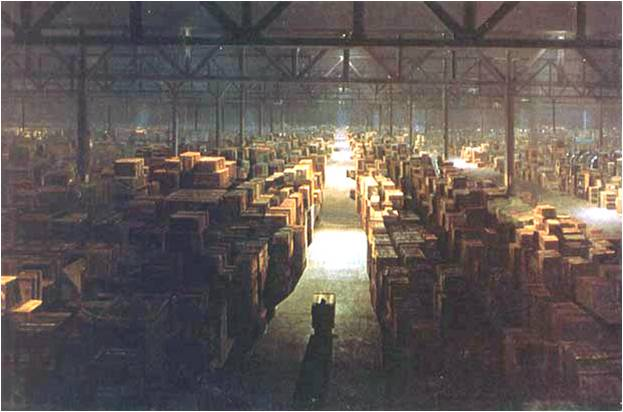
\includegraphics[width=0.6\textwidth]{images/indy-warehouse.jpg}
\end{center}

There is a crate for cURL, but it might be interesting to learn what one would have to do to use the C library for it...

\end{frame}



\end{document}

